% Copyright © 2017-2018 Martin Ueding <martin-ueding.de>
% Licensed under CC-BY 4.0

\documentclass{scrartcl}

\pagestyle{empty}

\usepackage{tikz}
\usetikzlibrary{arrows.meta, calc}

\colorlet{mygray1}{black!10}
\colorlet{mygray2}{black!20}

\begin{document}

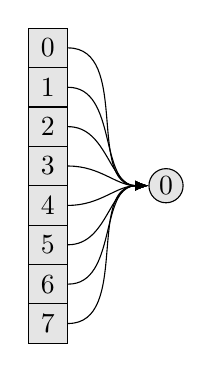
\begin{tikzpicture}[
        box/.style={
            draw,
            rectangle,
            minimum size=5mm,
        },
        block/.style={
            draw,
            circle,
            minimum size=0mm,
            inner sep=1.5pt,
        },
        marked/.style={
            fill=mygray1,
        },
        scale=0.5,
    ]

    \node[box, marked] (l0) at (0, -0) {0};
    \node[box, marked] (l1) at (0, -1) {1};
    \node[box, marked] (l2) at (0, -2) {2};
    \node[box, marked] (l3) at (0, -3) {3};
    \node[box, marked] (l4) at (0, -4) {4};
    \node[box, marked] (l5) at (0, -5) {5};
    \node[box, marked] (l6) at (0, -6) {6};
    \node[box, marked] (l7) at (0, -7) {7};

    \begin{scope}[xshift=30mm, yshift=-35mm]
        \node[block, marked] (b0) at (0, -0) {0};
    \end{scope}

    \begin{scope}[->, >=Latex, out=0, in=180]
        \draw (l0) to (b0);
        \draw (l1) to (b0);
        \draw (l2) to (b0);
        \draw (l3) to (b0);
        \draw (l4) to (b0);
        \draw (l5) to (b0);
        \draw (l6) to (b0);
        \draw (l7) to (b0);
    \end{scope}
\end{tikzpicture}

\end{document}
